%%%%%%%%%%%%%%%%%%%%%%%%%%%%%%%%%%%%%%
%% Frame
%%%%%%%%%%%%%%%%%%%%%%%%%%%%%%%%%%%%%%

\begin{frame}[t]
\frametitle{Introduction}
\framesubtitle{~~}  %% needed for proper positioning of the logo ...

The Basis pursuit problem 
\begin{equation}
min  \;||x||_{l_1} \qquad   subject \; to \; \Phi \Psi x=y
\end{equation}

\subsection*{Structured random matrices}
Toeplitz and Circulant matrices have the forms, respectively,
\\


$$
T = \begin{bmatrix}
	t_{n} & t_{n-1} & ...& t_{1}           \\[0.3em]
	t_{n+1} & t_n & ... & t_{2} \\[0.3em]
	\ddots &\ddots & \ddots &    \\[0.3em]
	t_{2n-1} & t_{2n-2}& ... & t_{n}         
\end{bmatrix}
\qquad and \qquad
C = \begin{bmatrix}
t_{n} & t_{n-1} & ...& t_{1}           \\[0.3em]
t_{1} & t_{n} & ... & t_{2} \\[0.3em]
\ddots &\ddots & \ddots &      \\[0.3em]
t_{n-1} & t_{n-2}& ... & t_{n}        
\end{bmatrix} 
$$
\end{frame}
%%%%%%%%%%%%%%%%%%%%%%%%%%%%%%%%%%%%%
%% Frame
%%%%%%%%%%%%%%%%%%%%%%%%%%%%%%%%%%%%%%
\begin{frame}[t]
	\frametitle{Structured random matrices}
	 Hadamard matrix is a square matrix whose entries are either $+1$ or $−1$ and whose rows are mutually orthogonal.
\begin{figure}[h]
\centering
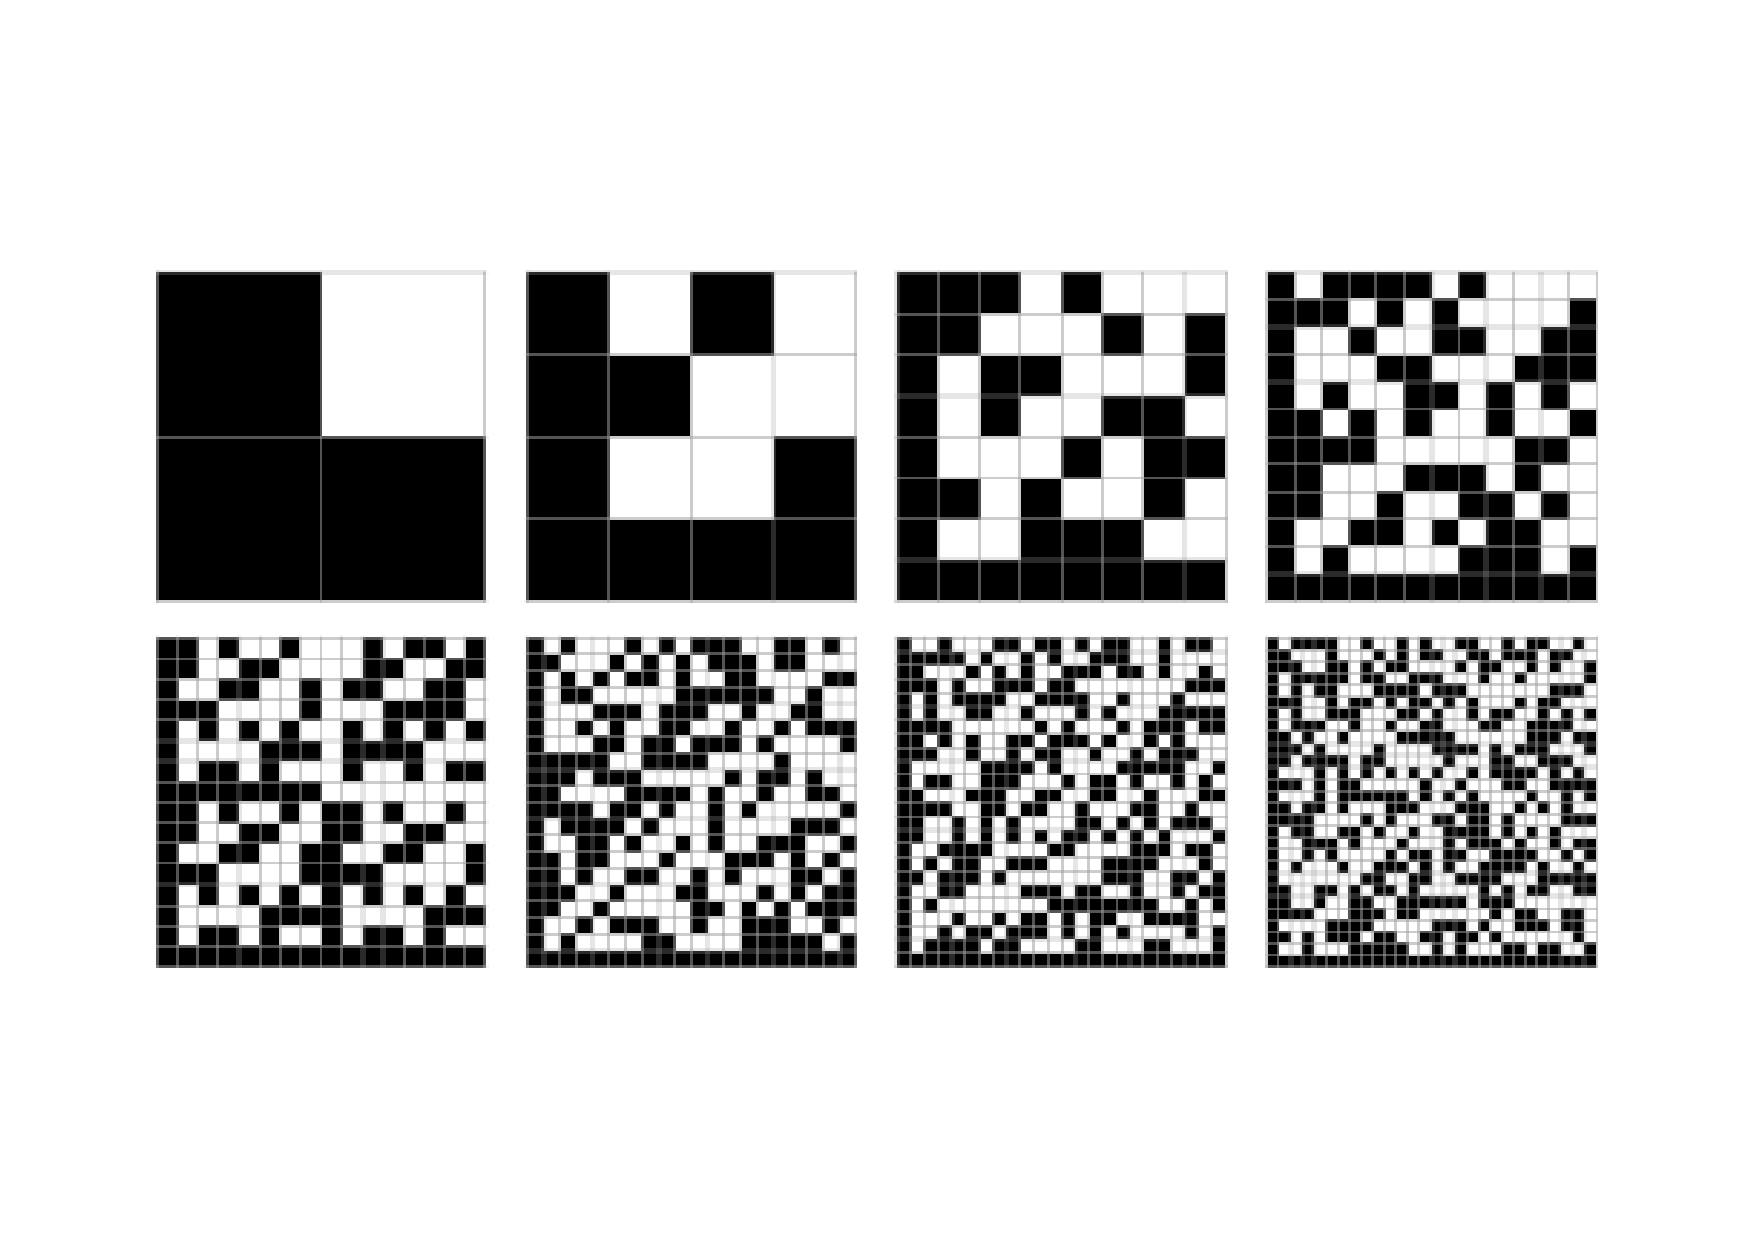
\includegraphics[width=0.7\linewidth]{HadamardMatrices_800}
\caption{}
\label{fig:HadamardMatrices_800}
\end{figure}

\end{frame}
%%%%%%%%%%%%%%%%%%%%%%%%%%%%%%%%%%%%%%
%% Frame
%%%%%%%%%%%%%%%%%%%%%%%%%%%%%%%%%%%%%%
\begin{frame}[t]
	\frametitle{Structured random matrices}
	An equivalent definition of the Hadamard matrices is given by 
	$$H_{n}H_{n}^T=nI_{n} $$
	where $I_{n}$ is the $n \times n$ identity matrix.
$$
	H_{1} = \begin{bmatrix}
		1
		\end{bmatrix}
\qquad
H_{2} = \begin{bmatrix}
1 & 1           \\[0.3em]
1& -1\\[0.3em]
\end{bmatrix}	
\qquad
H_{4} = \begin{bmatrix}
H_{2} & H_{2}           \\[0.3em]
H_{2}& -H_{2}\\[0.3em]
\end{bmatrix}	
\\
\centering
\qquad
H_{2^n} = \begin{bmatrix}
H_{2^{n-1}} & H_{2^{n-1}}           \\[0.3em]
H_{2^{n-1}}& -H_{2^{n-1}}            \\[0.3em]
\end{bmatrix}	


$$
	
	
\end{frame}




        
